\documentclass{letnab}
\pagestyle{fancy}
\usepackage{tabu}
\usepackage{units}
\usepackage{lscape}

\rhead{Общая физика МФТИ}
\lhead{Лабораторная работа 1.3.3} 

\renewcommand{\headrulewidth}{2pt}
\begin{document}
	\large

	\begin{titlepage}
		
		
		
		\center % Center everything on the page
		
		
		
		%----------------------------------------------------------------------------------------
		%	HEADING SECTIONS
		%----------------------------------------------------------------------------------------
		
		\textsc{\LARGE Московский Физико-Технический Институт}\\[1,5cm] % Name of your university/college
		% Major heading such as course name
		\textsc{\Large Кафедра общей физики}\\[0.5cm]
		\textsc{\large Отчет о выполнении лабораторной работы \textnumero  2.1.1}\\[0.5cm] % Minor heading such as course title
		
		%----------------------------------------------------------------------------------------
		%	TITLE SECTION
		%----------------------------------------------------------------------------------------
		
		\HRule
		\\[0.4cm]
		{ \huge \bfseries Измерение удельной теплоёмкости воздуха при постоянном давлении}
		\\[0.2cm] % Title of your document
		\HRule
		\\[1.5cm]
		
		
		
		%----------------------------------------------------------------------------------------
		%	AUTHOR SECTION
		%----------------------------------------------------------------------------------------
		
		\begin{minipage}{0.7\textwidth}
			\begin{center} \large
				\emph{Автор:} Алексей \textsf{Домрачев} 615 группа
			\end{center}
		\end{minipage}
		\\[1.0cm]
		\begin{minipage}{0.9\textwidth}
			\begin{center} \large
				\emph{Преподаватель:} Александр Дмитриевич \textsf{Калашников} % Supervisor's Name
			\end{center}
		\end{minipage}
		\vfill 
	%	\begin{bottompar}
			
\includegraphics[width = 80 mm]{logo.png}	\\[1,0cm]
			{\large \today}
	%	\end{bottompar}
		% Fill the rest of the page with whitespace
		
	\end{titlepage}


\section{Начальные сведения}
\subsection*{Цель работы}
\begin{enumerate}
\item Экспериментально выявить участок сормированного течения;
\item Определить режимы ламинарного и турбулентного течения;
\item Определить число Рейнольдса
\end{enumerate}
\subsection*{В работе используются}
\par Металлические трубки, укрепленные на горизонтальной подставке; газовый счетчик; микроманометр типа ММН; стеклянная U-образная трубка; секундомер.

\subsection*{Экспериментальная установка}
\begin{figure}[H]
	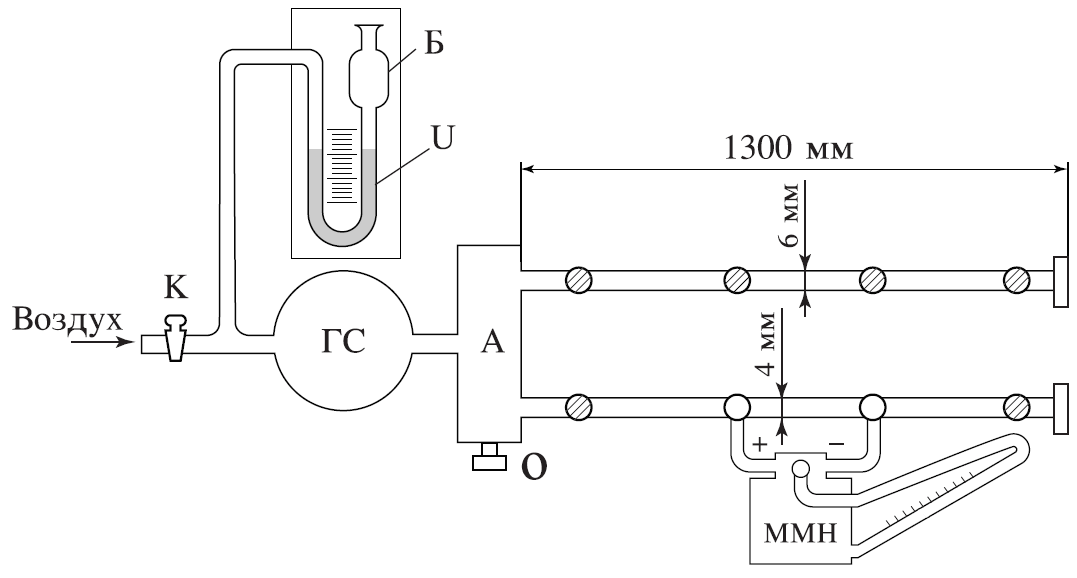
\includegraphics[width = 150 mm]{the_station.png}
	\caption{Схема установки для определения вязкости воздуха}
\end{figure}

Данная работа предусматривает следующую методику измерений в несколько этапов:
\begin{enumerate}
	\item Измерение вязкости воздуха: выбирается труба, на которой будут производиться измерения, к двум соседним участкам выбранной трубы, которые выбираются при условии того, что на них успевает сформироваться воздушный поток, подключается микроманометр. Далее снимается зависимость разности давлений $\Delta P$ от расхода воздуха $Q$.
	\item При расходе, заведомо обеспечивающем ламинарность потока, измеряется распределение давления вдоль всех трех трубок.
	\item Для всех трубок на участках со сформированным течением в ламинарном режиме снимаются зависимости $Q = f(P)$. 
\end{enumerate}
\section{Измерения и расчеты}
\par Оценим расстояние, на котором происходит формирование потока при ламинарном течении для выбранной трубки: $a = 0.2 r \cdot Re = 390 \text{ мм}$.
\begin{table}[H]
	\centering
	\caption{Расход воздуха и разность давлений в режиме ламинарного течения}
	\begin{tabu} to 0.9\textwidth {| c  || X[c] | X[c] | X[c] | X[c] | X[c] | X[c] |}
		\hline
		\textnumero & 1 & 2 & 3 & 4 & 5 & 6\\ \hline
		$\Delta V\text{, л}$  & 5 & 5 & 5 & 8 & 10 & 10 \\ \hline
		$\Delta t\text{, с}$  & 113.92 & 80.74 & 67.74 & 97.63 & 106.33 & 96.79\\ \hline
		$Q \cdot 10^2\text{, }\nicefrac{\text{л}}{\text{с}}$ & 4.39 & 6.19 & 7.38 & 8.19 & 9.40 & 10.33 \\ \hline
		$\Delta P \cdot 0.2 \text{, дел.}$  & 6.0 & 8.4 & 10.2 & 11.8 & 14.0 & 17.8  \\ \hline
		$\Delta P\text{, Па}$ & 11.78 & 16.48 & 20.01 & 23.14 & 27.46 & 34.91 \\ \hline
	\end{tabu}
\end{table}
\begin{table}[H]
	\centering
	\caption{Расход воздуха и разность давлений в режиме турбулентного течения}
	\begin{tabu} to 0.9\textwidth {| c  || X[c] | X[c] | X[c] | X[c] |}
		\hline
		\textnumero & 1 & 2 & 3 & 4 \\ \hline
		$\Delta V\text{, л}$  & 10  & 13 & 14 & 16\\ \hline
		$\Delta t\text{, с}$  & 88.24 & 106.24 & 102.06 & 103.70 \\ \hline
		$Q \cdot 10^2\text{, }\nicefrac{\text{л}}{\text{с}}$ & 11.33 &  12.24 & 13.72 & 15.43 \\ \hline
		$\Delta P \cdot 0.2 \text{, дел.}$  & 22.6 & 27 & 34.2 & 42.8  \\ \hline
	\end{tabu}
\end{table}
С помощью полученных данных и МНК рассчитаем угловой коэффициент наклона линейной части графика.
\begin{equation} 
k = \frac{\langle xy \rangle }{\langle x^2 \rangle} = \frac{7.49\cdot 10^{-3}}{6.24\cdot 10^{-9}} = 1200173
\end{equation}
\begin{equation} 
\sigma_k = \frac{1}{\sqrt{n}}\sqrt{\frac{\langle y^2 \rangle}{\langle x^2 \rangle} - k^2} = \frac{1}{\sqrt{6}} \sqrt{\frac{9060.95}{6.24\cdot 10^{-9}}- 1200173^2} = 45538 
\end{equation}

\begin{figure}[H]
	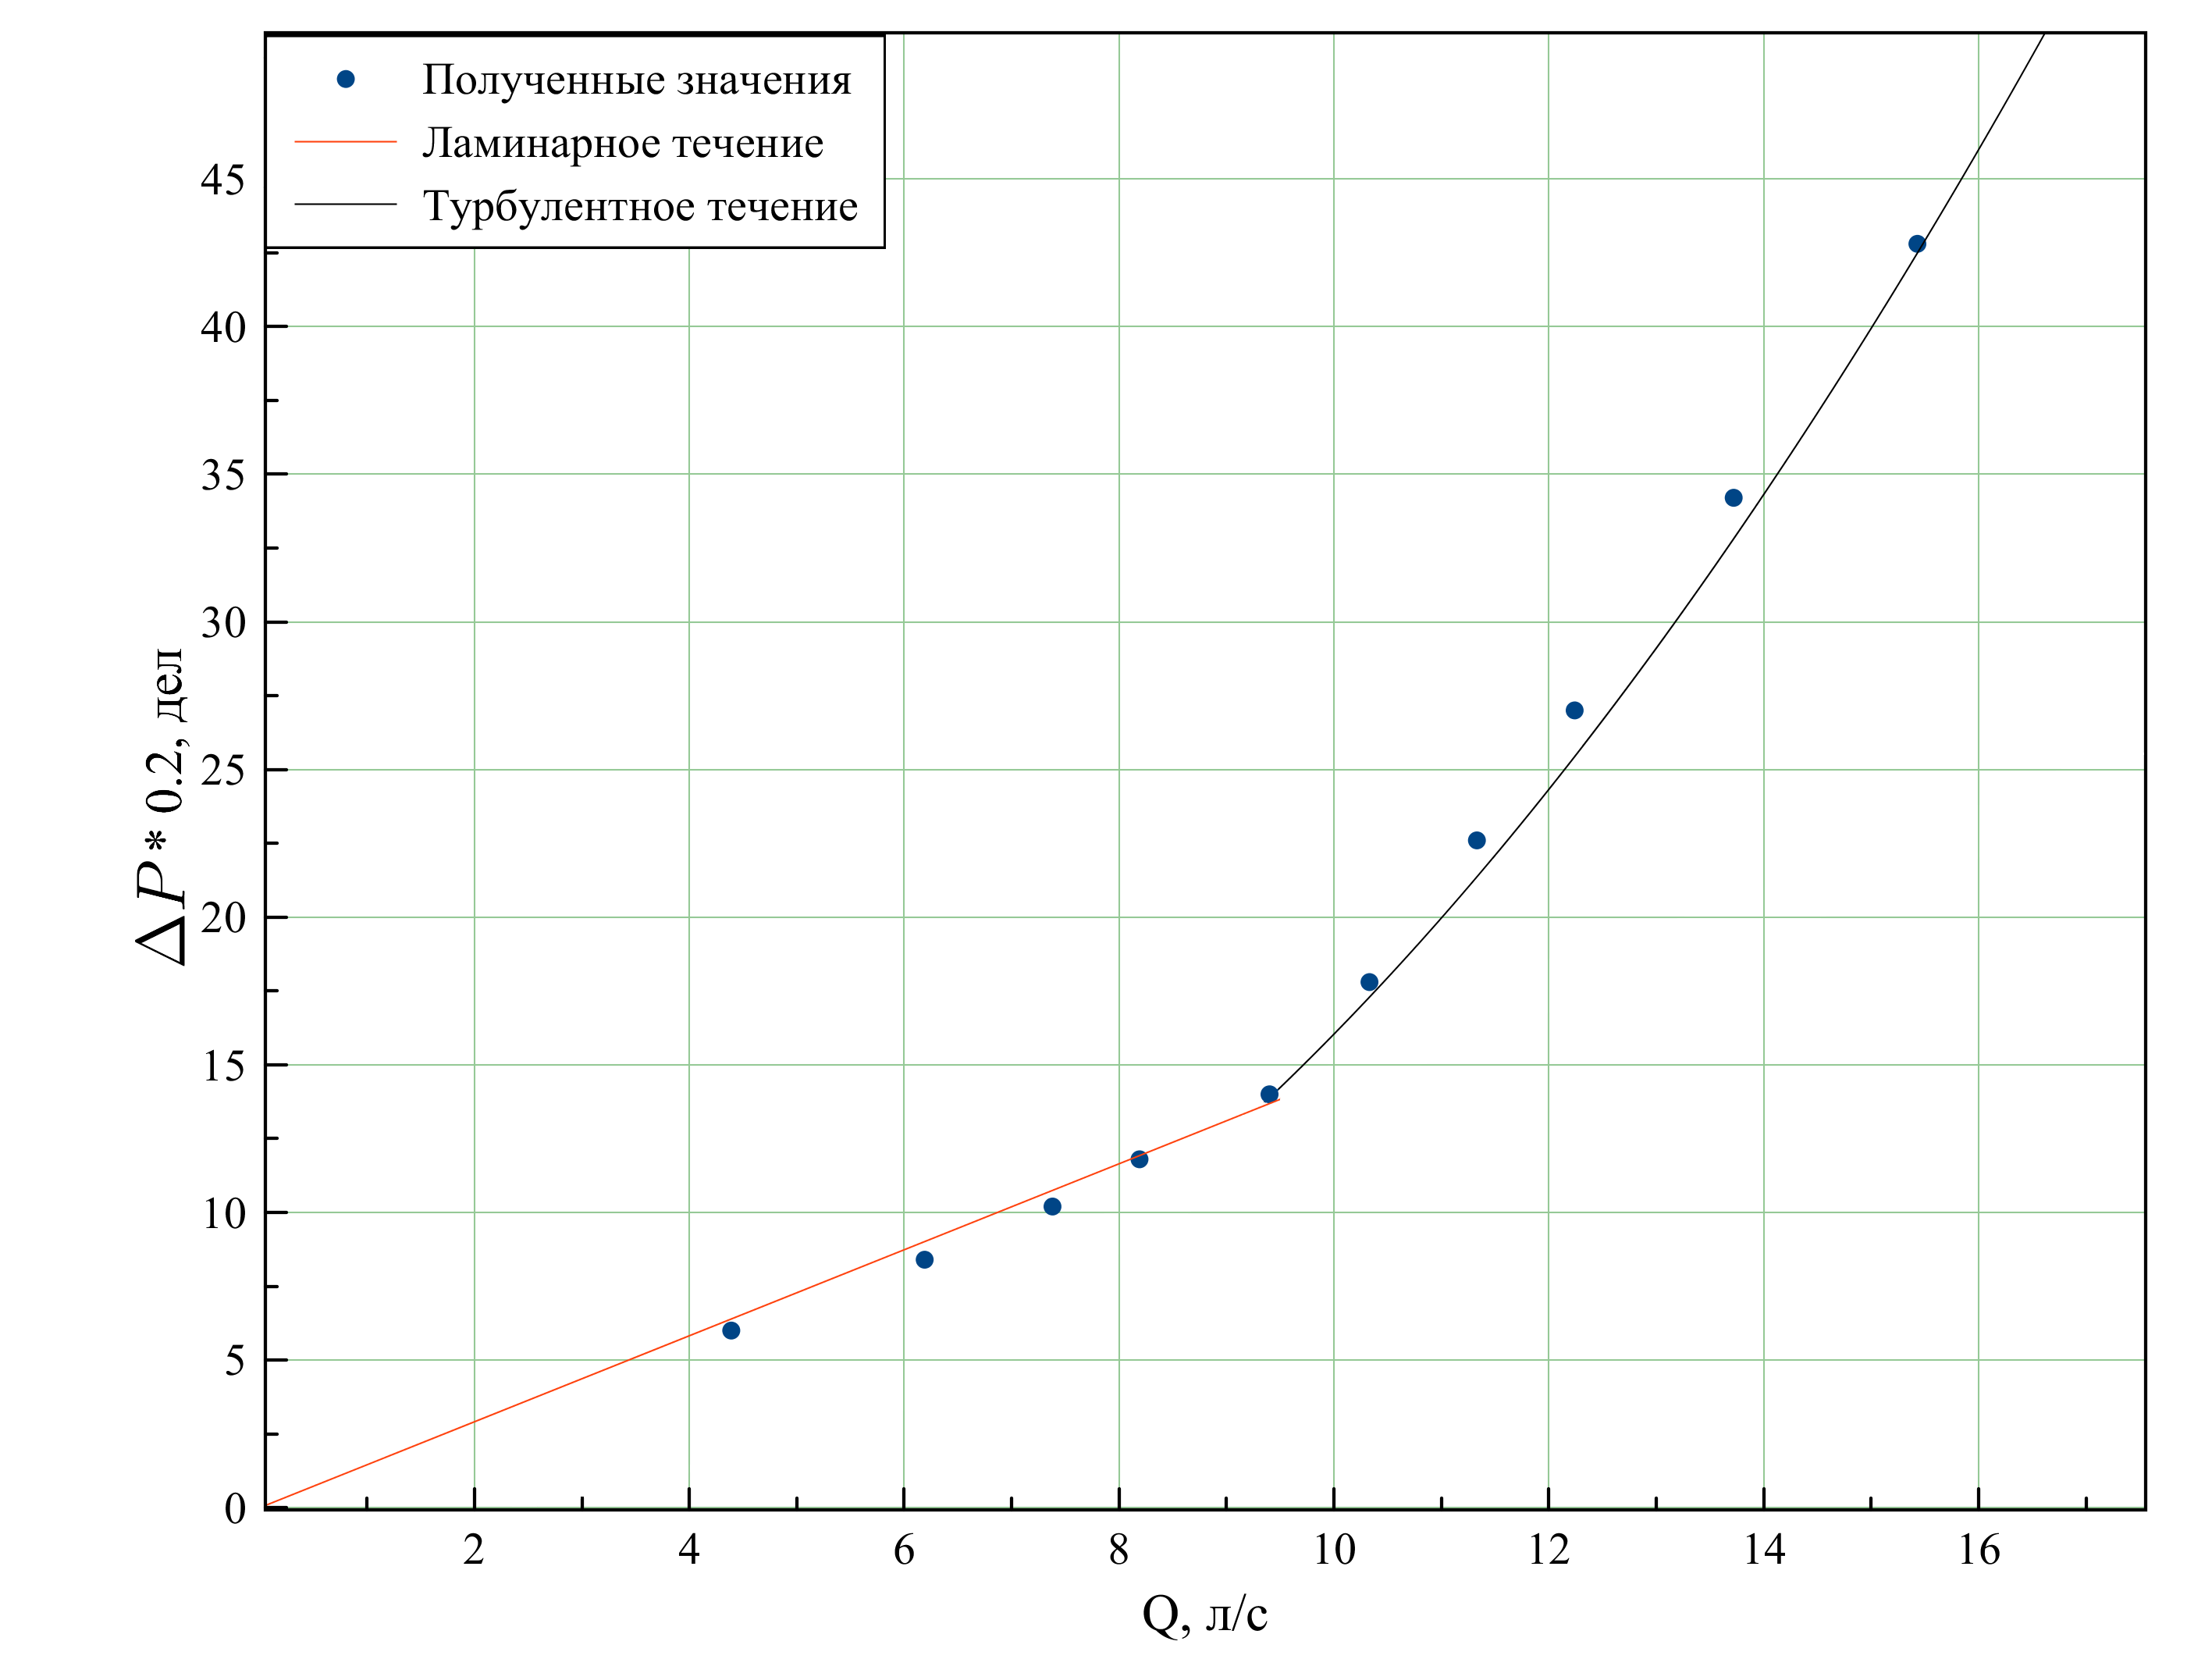
\includegraphics[width = 150 mm]{1.png}
	\caption{График зависимости $\Delta P$ от $Q$}
\end{figure}

Коэффициент вязкости воздуха вычислим с помощью формулы Пуазейля
\begin{equation} 
\eta = \frac{\pi r^4 k}{8l} = \frac{\pi \cdot 3.90^4 \cdot 1200173}{8 \cdot 0.5 \cdot 2^4 \cdot 10^{12}} = 13.6 \cdot 10^{-6} \, \text{Па} \cdot \text{с}
\end{equation}
Подсчитаем ошибку:
\begin{equation}
\sigma_\eta = \eta \sqrt{16\left(\frac{\sigma_r}{r}\right)^2+\left(\frac{\sigma_k}{k}\right)^2}=0.9\cdot 10^{-6} \,\text{Па}\cdot\text{с}
\end{equation}
\huge Итог: \fbox{$\eta = 13.6 \pm 0.9 \cdot 10^{-6} \text{ Па}\cdot \text{с}$}\\
\normalsize \newpage
Значения $Q = 9.40\cdot 10^{-5}\, \nicefrac{\text{м}^3}{\text{с}}$ и $\Delta P =111.14 \,\text{Па}$ соответствуют значениям переходной области между ламинарным и турбулентным течением. Значение плотности воздуха возьмем $1.184 \,\nicefrac{\text{кг}}{\text{м}^3}$, т.к. это значение соответствует воздуху при нормальных условиях при $25 ^\circ C$. Рассчитаем значение числа $Re$ при этих данных:
\begin{equation}
v = \frac{Q}{S};\; Re = \frac{vr\rho}{\eta} = \frac{2Q\rho}{\eta \pi d} = \frac{2 \cdot 9.40 \cdot 10^{-5} \cdot 1.184}{13.6 \cdot 10^{-6} \cdot \pi \cdot 3.90 \cdot 10^{-3}} =1335
\end{equation} 

\begin{minipage}{8.5cm}
\begin{table}[H]
	\centering
	\caption{Зависимость давления от\\ длины~трубки при ламинарном течении}
	\begin{tabular}{|c|c|c|}
		\hline
		$l$, см & $Q_1 \cdot 10^2,\, \nicefrac{\text{л}}{\text{с}}$ & $\Delta P_1$, дел   \\ \hline
		10.5    &6.39  &32  \\ \hline
		40.5    &7.12  &71  \\ \hline
		80.5    &6.64  &107  \\ \hline
		130.5   &6.92  &155  \\ \hline
	\end{tabular}
\end{table}
\begin{figure}[H]
	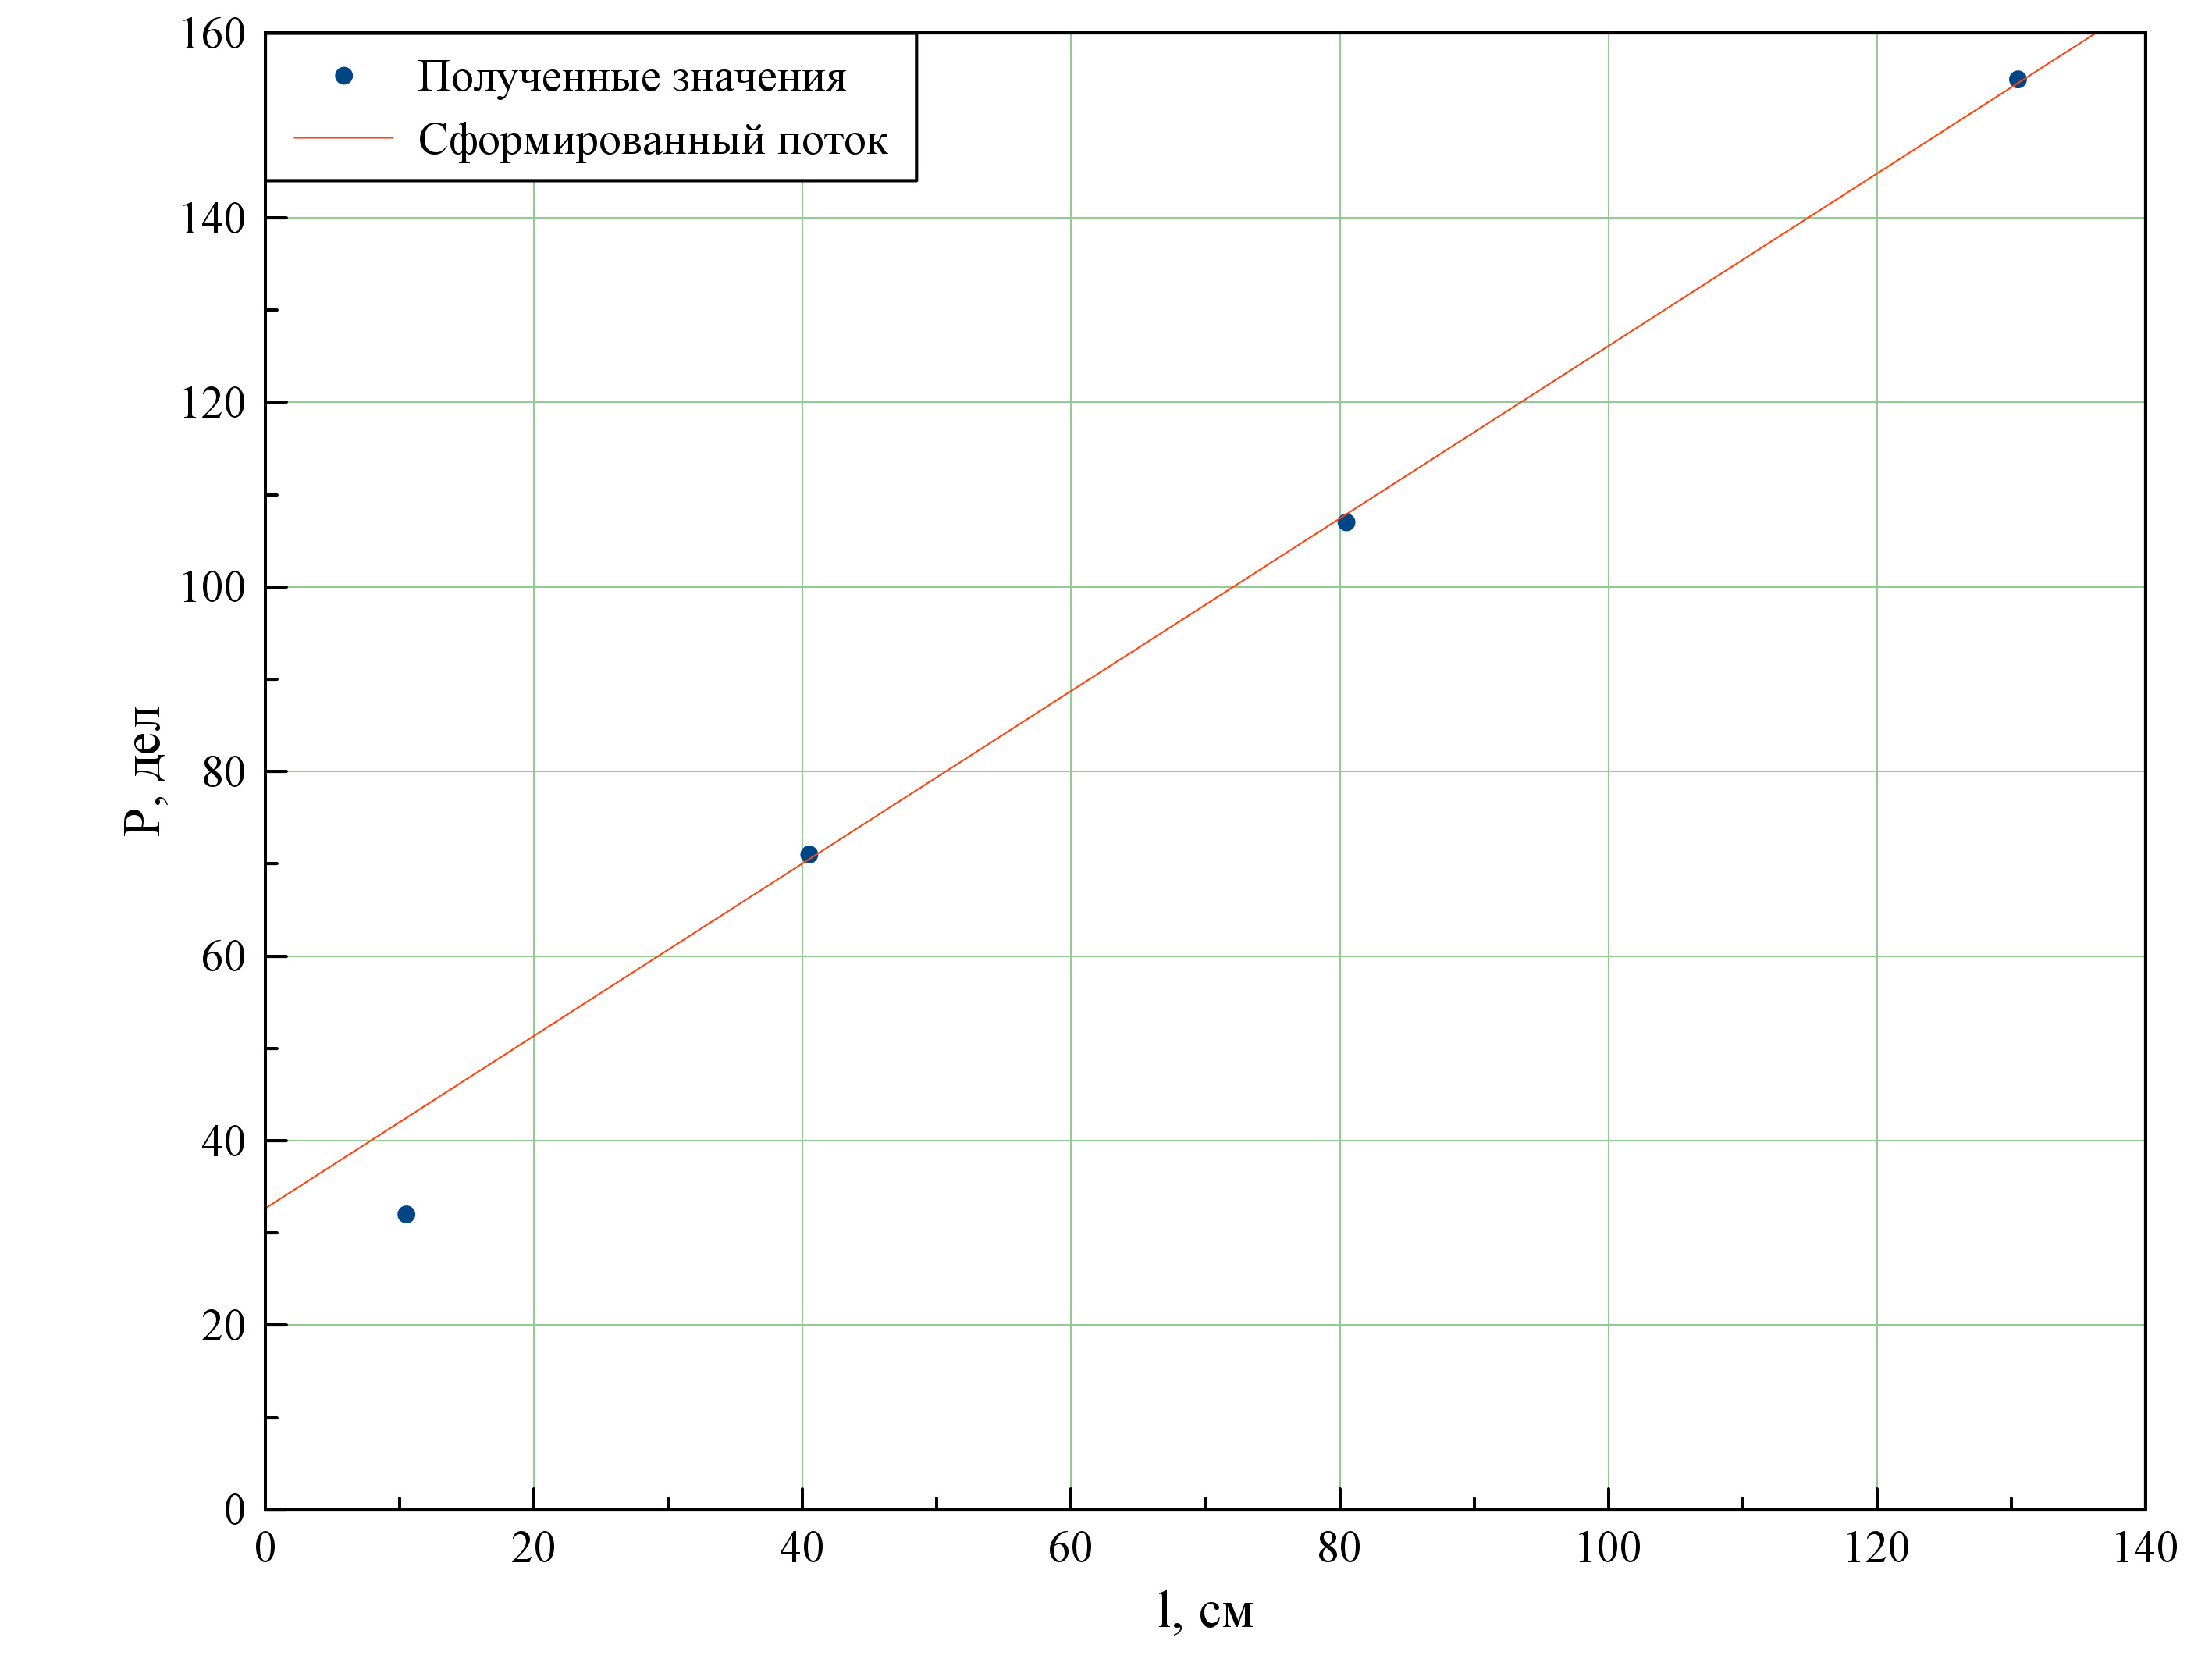
\includegraphics[width = 85 mm]{2.png}
	\caption{График зависимости $\Delta P$ от $l$}
\end{figure}
\end{minipage}
\begin{minipage}{8.5cm}
\begin{table}[H]
	\centering
	\caption{Зависимость давления от длины трубки на границе}
	\begin{tabular}{|c|c|c|}
		\hline
		$l$, см & $Q_2 \cdot 10^2 \nicefrac{\text{л}}{\text{с}}$ & $\Delta P_2$, дел   \\ \hline
		10.5    & 10.06     & 74                 \\ \hline
		40.5    & 10.91     & 151                \\ \hline
		80.5    & 10.47     & 239                \\ \hline
		130.5   & 9.48      & 264                \\ \hline
	\end{tabular}
\end{table}
\begin{figure}[H]
	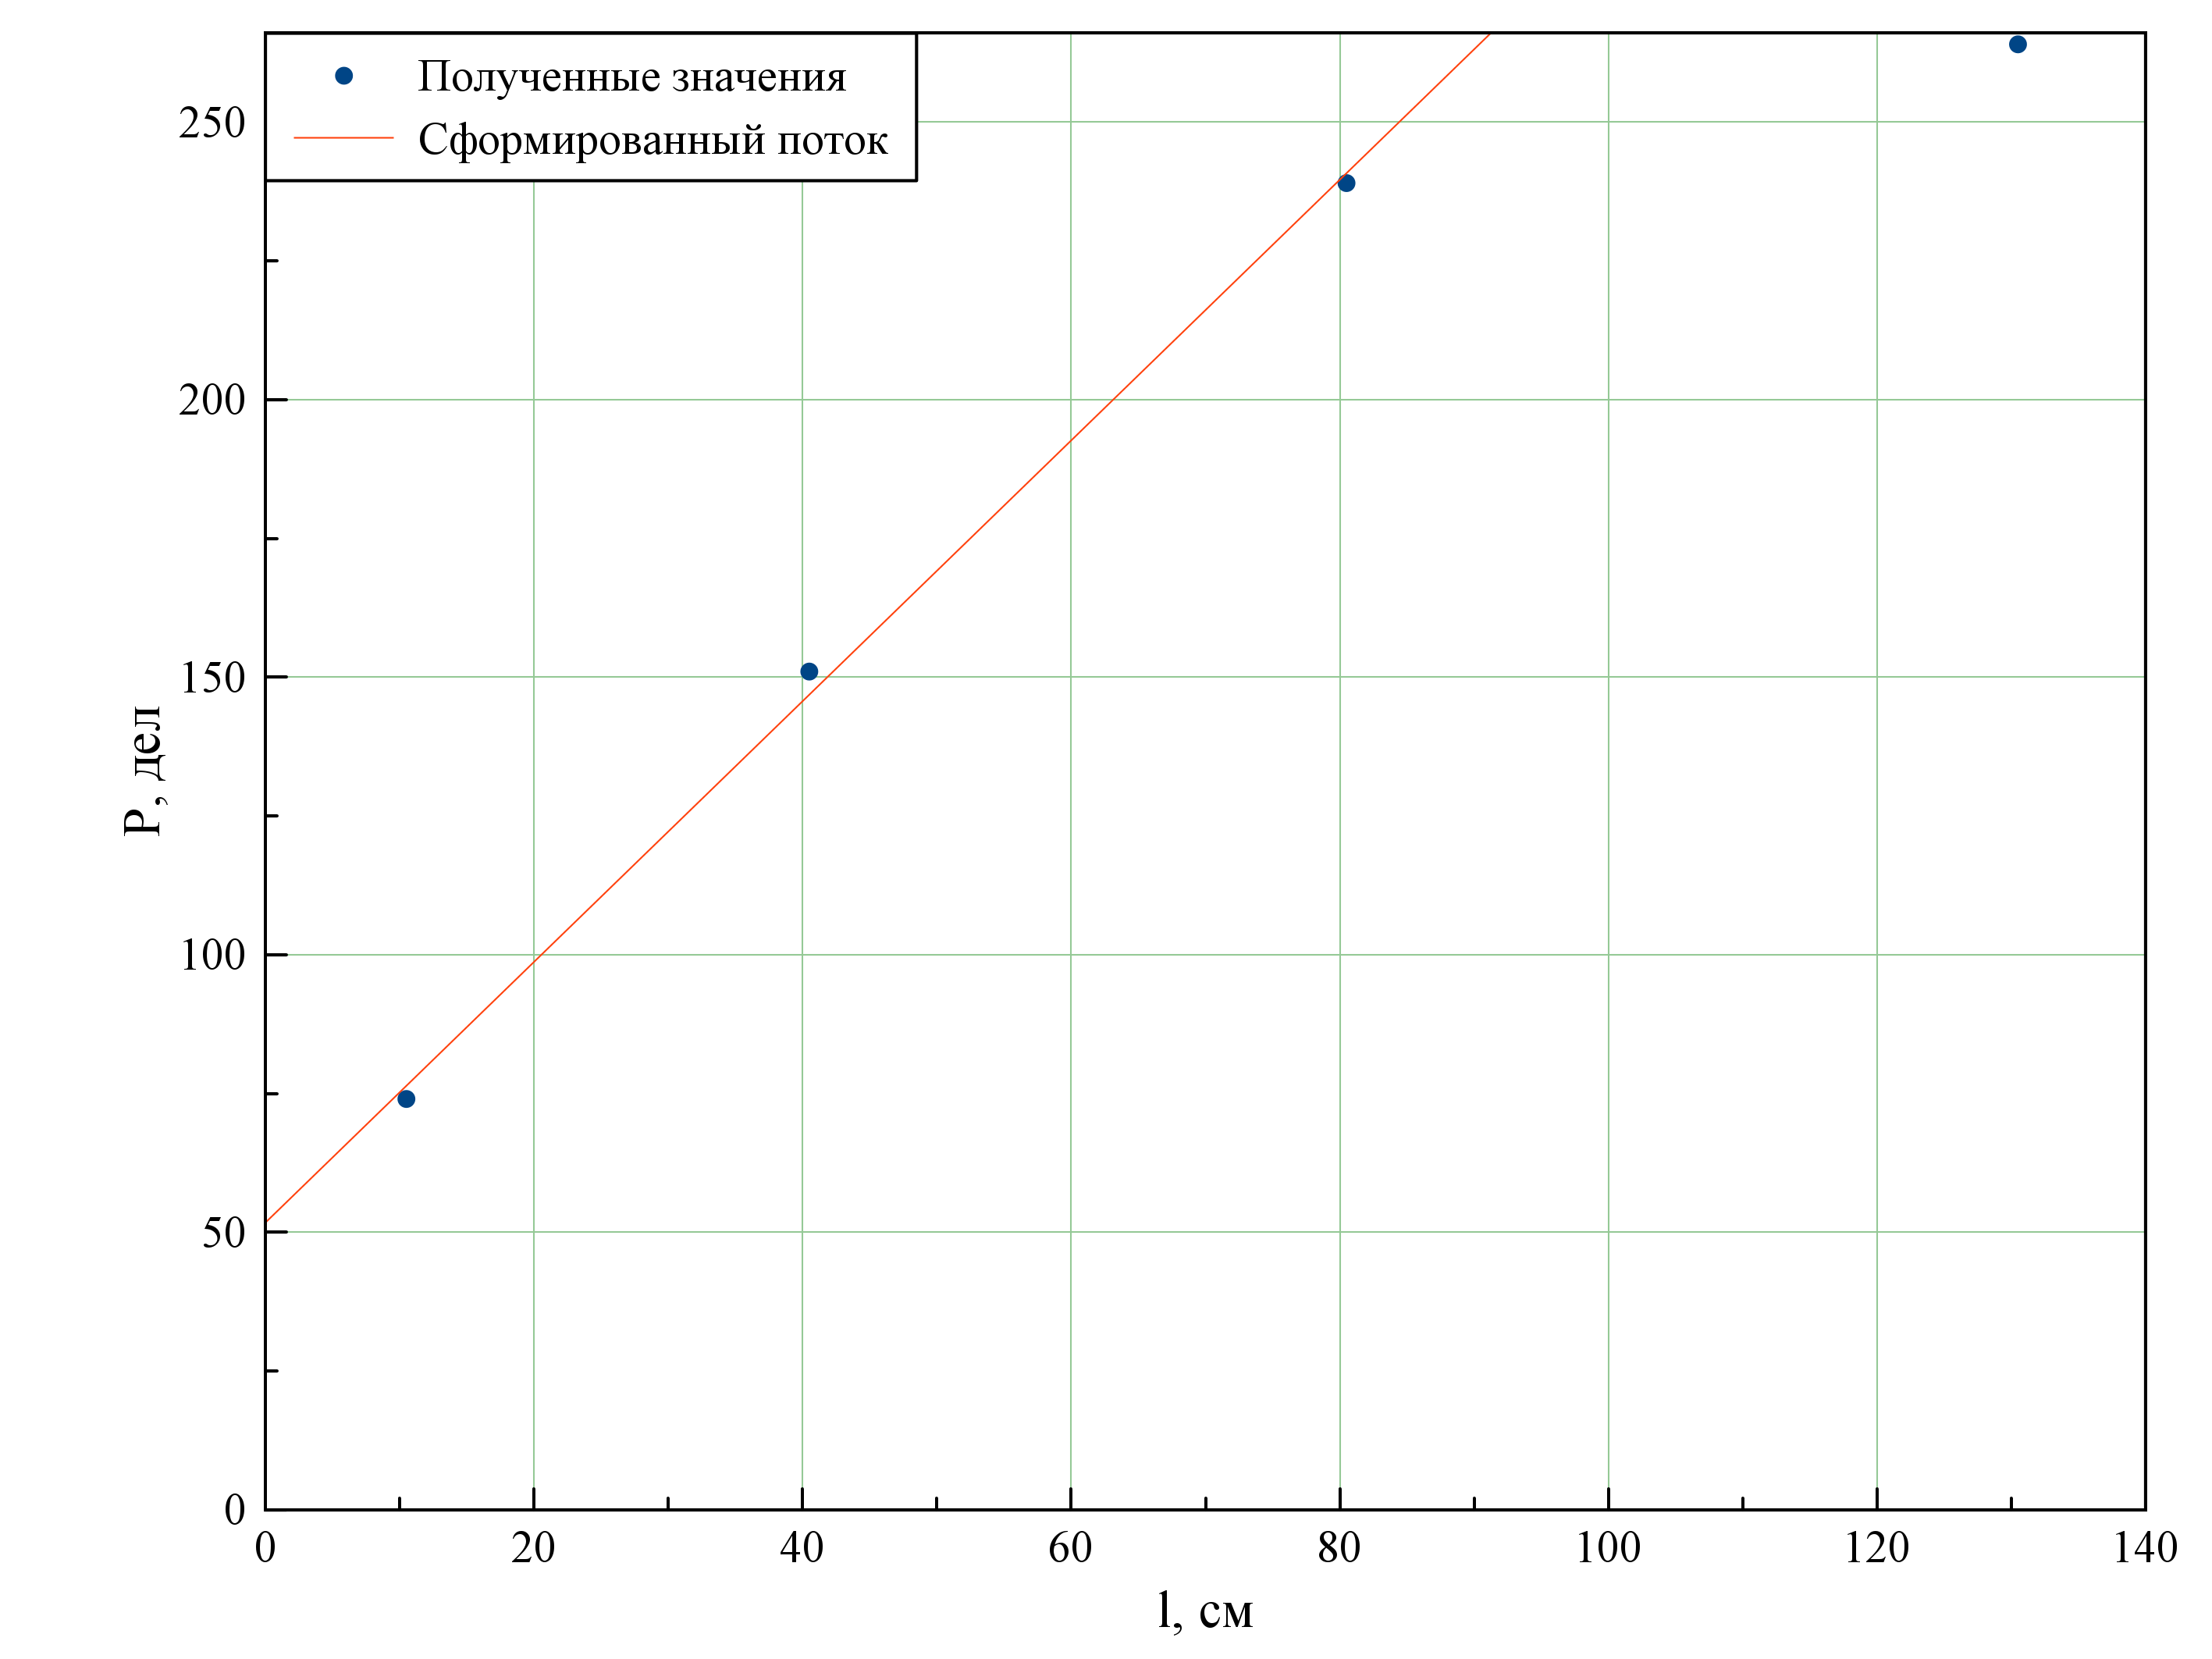
\includegraphics[width = 85 mm]{3.png}
	\caption{График зависимости $\Delta P$ от $l$}
\end{figure}
\end{minipage}
\\ \\
Из рисунка 3 мы видим, что поток воздуха сформировывается при $l \geqslant 40$~см, что соответствует полученным теоретическим вычислениям: $a=390$ мм.
\begin{table}[H]
	\centering
	\caption{}
	\begin{tabular}{|c|c|c|c|c|c|}
		\hline
		& $Q\cdot10^2$, $\nicefrac{\text{л}}{\text{с}}$ & $\Delta P$, дел & $r$, мм & $\ln r$ & $\ln r^n$\\ \hline
		\multirow{3}{*}{Труба 1} & 3.33 & 26 &\multirow{3}{*}{3.00} & \multirow{3}{*}{5.8091}  & 15.0898\\ \cline{2-3} \cline{6-6}  
		& 5.91 & 54 & & & 15.2481\\ \cline{2-3}  \cline{6-6}
		& 8.53 & 88 & & & 15.3695\\ \hline 
		\multirow{3}{*}{Труба 2} & 4.11 & 8 & \multirow{3}{*}{5.90} & \multirow{3}{*}{5.1328} & 13.5680 \\ \cline{2-3} \cline{6-6}
		& 9.85 & 12 & & & 13.2333\\ \cline{2-3} \cline{6-6} 
		& 18.25 & 55 & & & 14.1899 \\ \hline
	\end{tabular}
\end{table}
	С помощью полученных данных и МНК рассчитаем угловой коэффициент графика:
	\begin{equation}
	b = \frac{\langle xy\rangle - \langle x \rangle \langle y \rangle }{\langle x^2 \rangle - \langle x \rangle^2} = 2.35;\; \sigma_b = 0.33
	\end{equation}
$b \ne 4 \then$ эксперементальное значение степени $r$ не совпало с теоретическим.
\begin{figure}[H]
	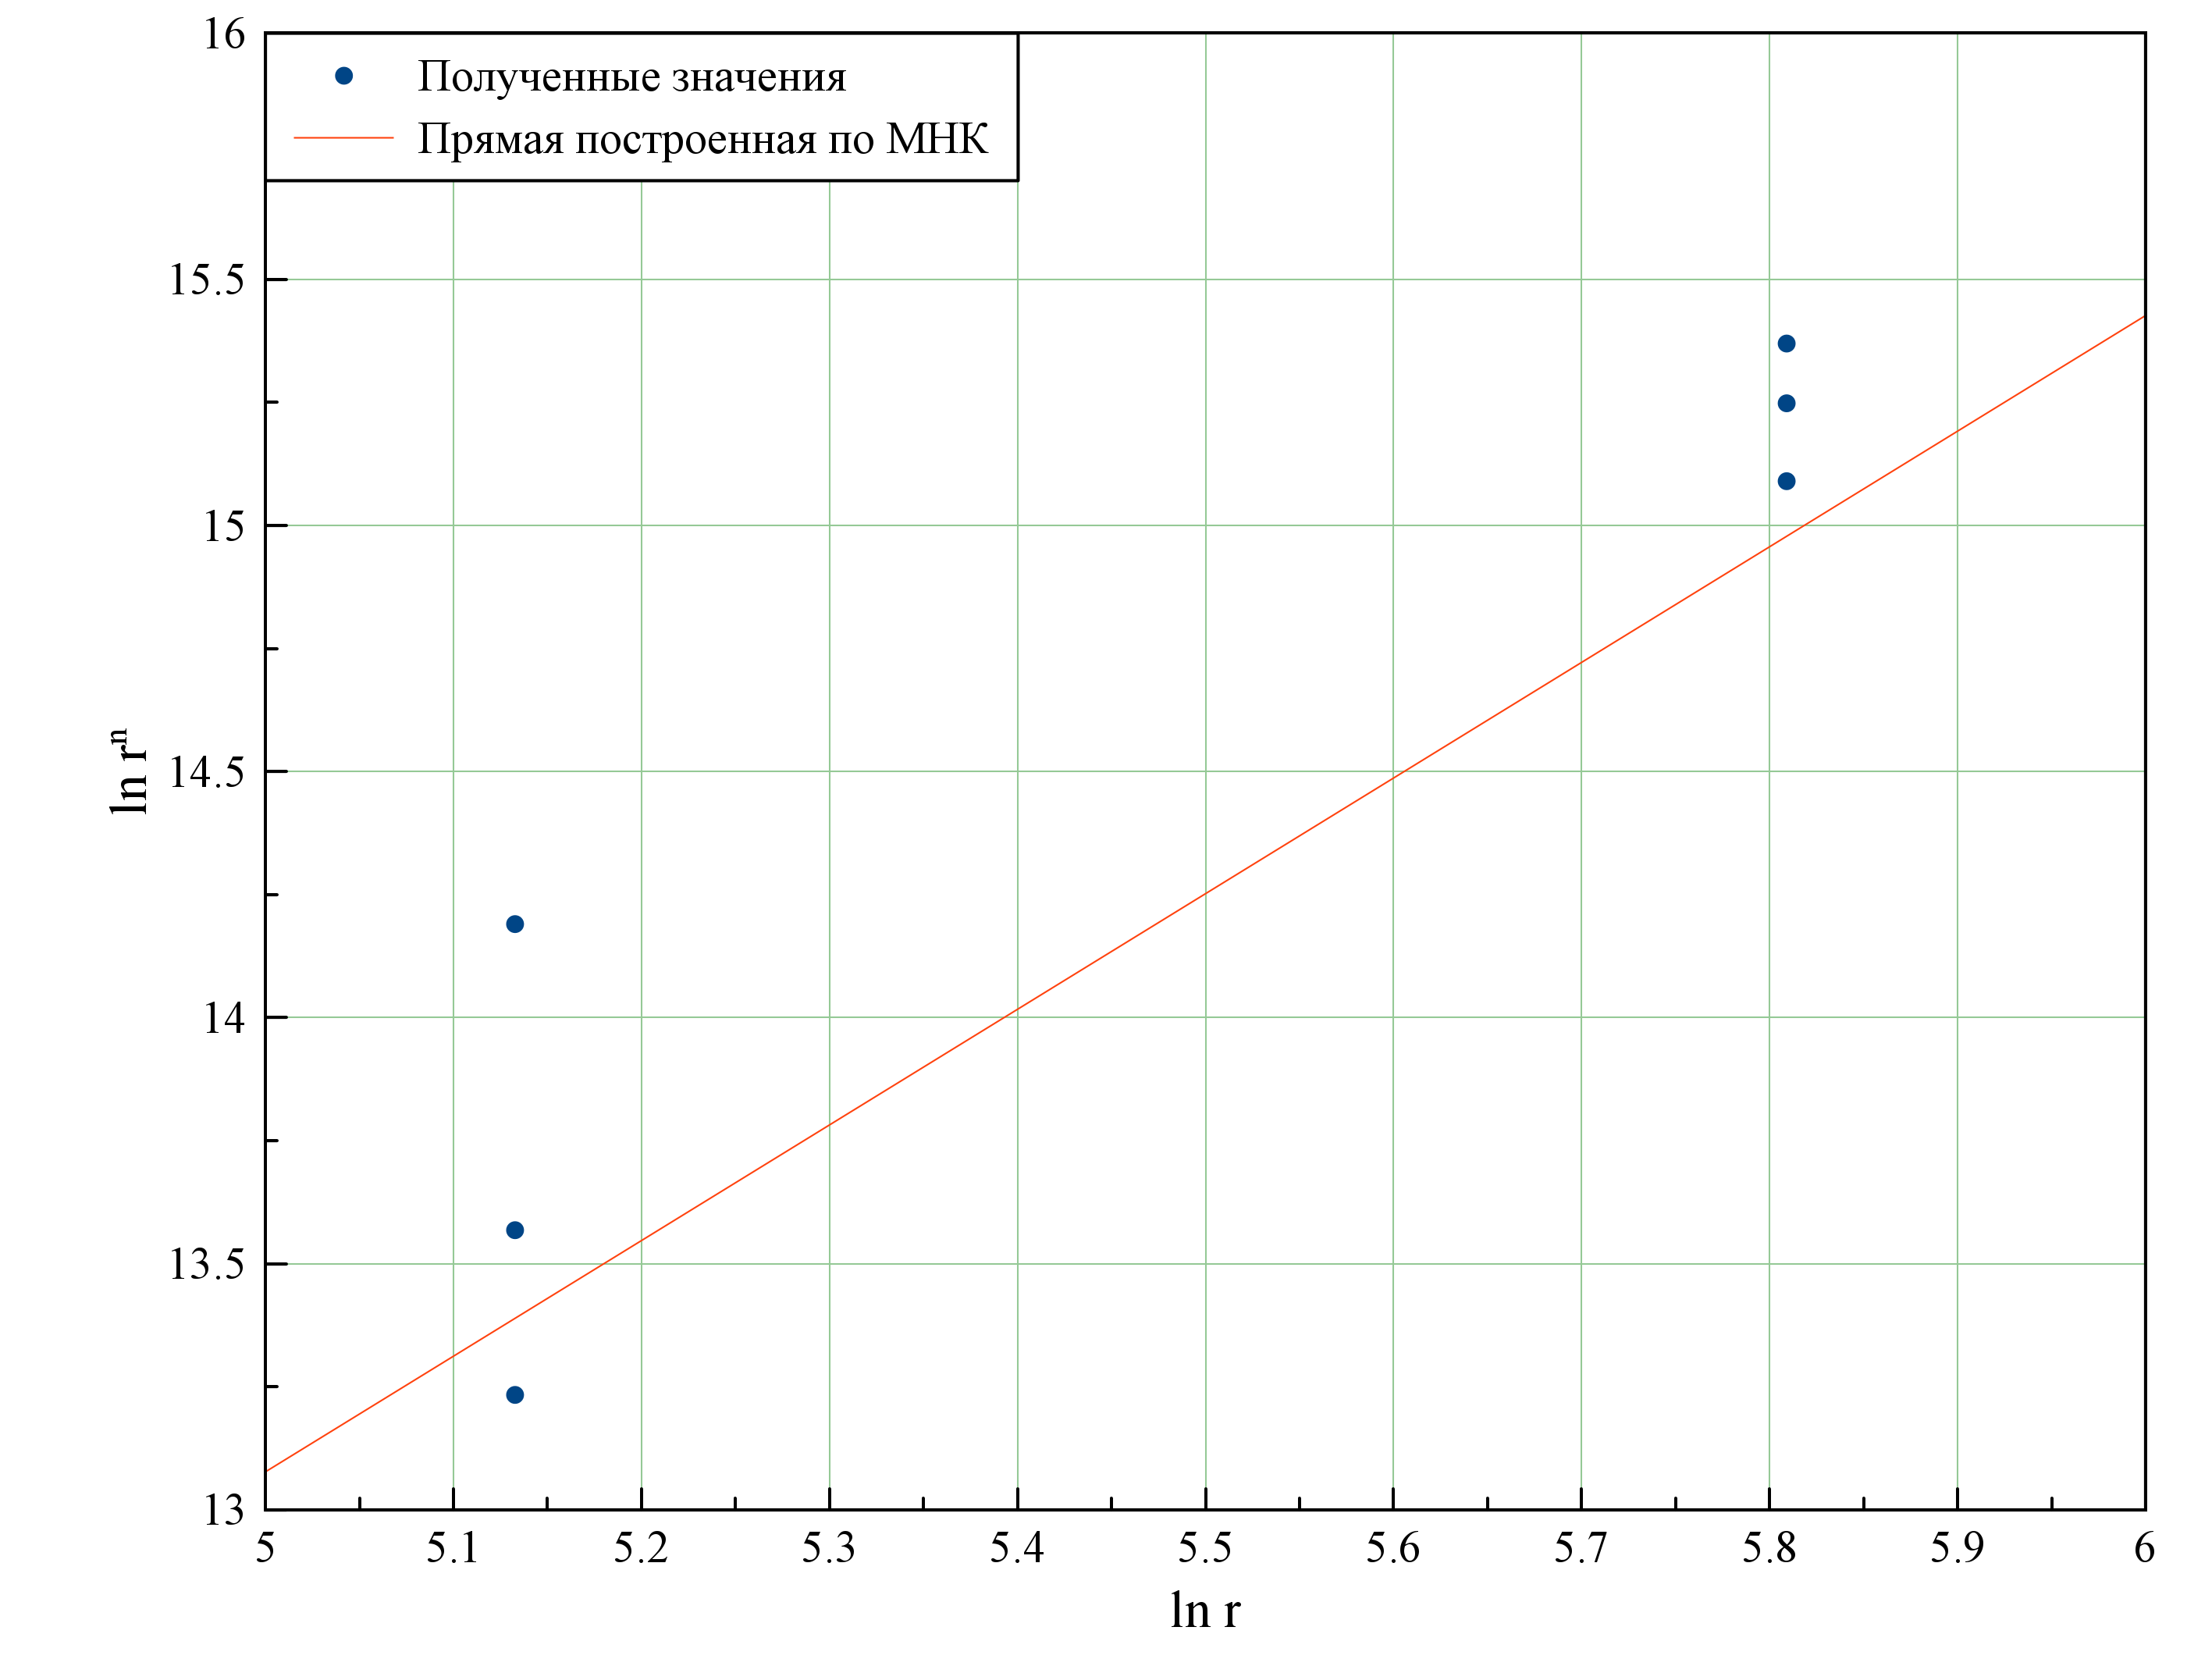
\includegraphics[width = 170 mm]{4.png}
	\caption{График зависимости $\ln r^n $ от $\ln r$}
\end{figure}
\section{Вывод}
\begin{enumerate}
	\item Практическое значение вязкости воздуха отличается от теоретического на 31\%.
	\item Мы проверили на практике, что режим воздушного потока устанавливается при длине трубы $>$ 40 см, что соответствует теоретическому значению 390 мм.
	\item Практическое значение n не сошлось с теоретическим 4. Так как эксперимент был проведен правильно, считаю что это неполадка оборудования.
\end{enumerate}
\end{document}